\newpage
\clearpage

\section{Resultados e Discussões}
\label{results}
Neste capítulo, dedicado a Resultados e Discussões, serão apresentados e analisados os resultados dos experimentos realizados no transcurso deste estudo, acompanhados de uma reflexão criteriosa sobre os dados obtidos. Nesta etapa, será possível, portanto, avaliar a eficácia dos métodos que foram propostos e implementados, além de discutir as ideias futuras de implementação e as perspectivas coletadas para a evolução do tema em questão.

A estrutura do capítulo é delineada em seções que facilitam a compreensão dos resultados de acordo com o contexto do experimento aplicado. Na Seção \ref{results:class}, será discutido sobre os experimentos realizados prioritariamente para a tarefa de classificação. Esses experimentos iniciais foram fundamentais para balizar as análises e refinamentos subsequentes da técnica proposta.

Na sequência, a Seção \ref{results:semantic} irá abordar os resultados obtidos nos experimentos que se destinam diretamente à área de segmentação, que constitui o núcleo da aplicação da técnica proposta. Aqui, expandiremos o foco para a parcela mais crítica de nossa pesquisa, apresentando a eficácia de nosso método na tarefa de segmentação semântica de imagens.

Por fim, na Seção \ref{result:final} proporcionaremos as considerações finais em relação as seções anteriores, salientando as implicações dos resultados no campo de estudo do trabalho.

\subsection{Resultados da Classificação de Imagens}
\label{results:class}
Os experimentos e resultados desta seção oferecem percepções valiosas sobre o desempenho do método BPCAPooling em comparação com as estratégias de pooling convencionais (\textit{Avg Pooling} e \textit{Max Pooling}) \citep{Ozdemir2023Avg-topk:Networks}. Adicionalmente, esta seção apresentará informações sobre a influência da aplicação dessas estratégias em diferentes conjuntos de dados (Seção \ref{results:class:datasets}), a exploração da interpretabilidade das classificações utilizando a abordagem LIME (Seção \ref{results:class:lime}), e sugestões para possíveis melhorias no desempenho do modelo atual (Seção \ref{results:class:future}).

O desempenho do modelo treinado no conjunto de dados CIFAR-100 utilizando o método proposto apresentou a maior perda e o menor valor de precisão, o que não é desejado, e o modelo utilizando \textit{Max Pooling} obteve os melhores resultados, como pode ser observado na Tabela \ref{tab:cifar_values}.

\begin{table}[H]
    \caption{Results based on a CIFAR-100 warm-up}
    \label{tab:cifar_values}
    \centering
    \begin{tabular}{lcc}
        \firsthline
        \textbf{Pooling Methods} & \textbf{Accuracy (\%)} & \textbf{Loss}   \\
        \hline
        AvgPooling               & 36.300                 & 2.7309          \\
        BPCAPooling              & 14.471                 & 3.7645          \\
        MaxPooling               & \textbf{39.857}        & \textbf{2.0481} \\
        \lasthline
    \end{tabular}
\end{table}

Mesmo no processo de \textit{fine-tuning} o modelo treinado no conjunto de dados CIFAR 100 apresenta resultados inferiores, como demonstrado na Tabela \ref{tab:cifar_finetuning}, em que os métodos \textit{Max Pooling} e \textit{Avg Pooling} continuam se demonstrando significativamente superiores em relação ao método BPCAPooling, mas um dos grandes motivos dessa situação serão discorridos na Seção \ref{results:class:datasets}.

\begin{table*}[htbp]
    \caption{Fine-tuning results of various pooling methods on the CIFAR-100 dataset, categorized by blocks.}
    \label{tab:cifar_finetuning}
    \centering
    \begin{tabular}{lllllllll}
    \firsthline
    \multicolumn{1}{c}{\textbf{Pooling Methods}} & \multicolumn{2}{c}{\textbf{Warm-up}}                                          & \multicolumn{2}{c}{\textbf{Block 5}}                                          & \multicolumn{2}{c}{\textbf{Block 4}}                                          & \multicolumn{2}{c}{\textbf{Block 3}}                                          \\
    \cline{2-9}
    \multicolumn{1}{c}{\textbf{}}                & \multicolumn{1}{c}{\textbf{Accuracy(\%)}} & \multicolumn{1}{c}{\textbf{Loss}} & \multicolumn{1}{c}{\textbf{Accuracy(\%)}} & \multicolumn{1}{c}{\textbf{Loss}} & \multicolumn{1}{c}{\textbf{Accuracy(\%)}} & \multicolumn{1}{c}{\textbf{Loss}} & \multicolumn{1}{c}{\textbf{Accuracy(\%)}} & \multicolumn{1}{c}{\textbf{Loss}} \\
    \hline
    AvgPooling                                   &                                    36.300 &                            2.7309 &                                    39.340 &                            2.4971 &                                    41.371 &                            2.2958 &                                    42.371 &                            2.2364 \\
    BPCAPooling                                  &                                    14.471 &                            3.7645 &                                    15.185 &                            3.6677 &                                    16.229 &                            3.6020 &                                    17.543 &                            3.5121 \\
    MaxPooling                                   &                                    39.857 &                            2.0481 &                                    43.671 &                            1.7166 &                                    45.100 &                            1.5448 &                                    \textbf{46.071} &                            \textbf{1.4862} 
    \end{tabular}
\end{table*}

Para o conjunto de dados \textit{Food}-101, os resultados também não foram discrepantes quando comparado ao primeiro conjunto de dados, haja vista que logo na fase de aquecimento os resultados já se paresentam muito inferiores quando comparado aos demais métods, o que pode ser visualizado pela representação da Tabela \ref{}.

\begin{table}[htbp]
    \caption{Results based on a Food-101 warm-up}
    \label{tab:food_values}
    \centering
    \begin{tabular}{lcc}
        \firsthline
        \textbf{Pooling Methods} & \textbf{Accuracy (\%)} & \textbf{Loss}   \\
        \hline
        AvgPooling               & 41.290                 & 2.4042          \\
        BPCAPooling              & 41.426                 & 2.3863          \\
        MaxPooling               & \textbf{41.623}        & \textbf{2.3718} \\
        \lasthline
    \end{tabular}
\end{table}

Quanto a aplicação do processo de \textit{fine-tuning}, pode se perceber que em todas as fases o modelo de \textit{pooling} proposto se apresentou inferior, tendo a evolução do processo de \textit{fine-tuning} representada na Tabela \ref{tab:food_finetuning}, todavia mesmo com os resultados inesperados alguns insights poderam se obtidos por meio das fases de treinamento e validação, os quais serão comentados nas próximas seções.

\begin{table*}[htbp]
    \caption{Fine-tuning results of various pooling methods on the Food-101 dataset, categorized by blocks.}
    \label{tab:food_finetuning}
    \centering
    \begin{tabular}{lllllllll}
    \firsthline
    \multicolumn{1}{c}{\textbf{Pooling Methods}} & \multicolumn{2}{c}{\textbf{Warm-up}}                                          & \multicolumn{2}{c}{\textbf{Block 5}}                                          & \multicolumn{2}{c}{\textbf{Block 4}}                                          & \multicolumn{2}{c}{\textbf{Block 3}}                                          \\
    \cline{2-9}
    \multicolumn{1}{c}{\textbf{}}                & \multicolumn{1}{c}{\textbf{Accuracy(\%)}} & \multicolumn{1}{c}{\textbf{Loss}} & \multicolumn{1}{c}{\textbf{Accuracy(\%)}} & \multicolumn{1}{c}{\textbf{Loss}} & \multicolumn{1}{c}{\textbf{Accuracy(\%)}} & \multicolumn{1}{c}{\textbf{Loss}} & \multicolumn{1}{c}{\textbf{Accuracy(\%)}} & \multicolumn{1}{c}{\textbf{Loss}} \\
    \hline
    MaxPooling                                  &                                    41.623 &                            2.3718 &                                    49.471 &                            2.2033 &                                    50.080 &                            2.3745 &                                    50.031 &                            2.4335 \\
    BPCAPooling                                   &                                    41.426 &                            2.3863 &                                    49.556 &                            2.1862 &                                    \textbf{50.234} &                            \textbf{2.3820} &                                    50.139 &                            2.4474 
    \end{tabular}
\end{table*}

\subsubsection{Diferença de conjuntos de dados}
\label{results:class:datasets}
O uso de mais de um conjunto de dados foi de extrema importância para o atual estudo, visto que a quantidade de informação teve um grande impacto na quantidade de detalhes e características que a rede VGG-16 pôde captar, comportamento que vai diretamente em relação à motivação de uso das CNNs, como citado na Seção \ref{cnn}. Sendo assim, a partir da Figura \ref{results:fig:datasets:1} é possível visualizar a diferença de resolução de uma amostra do conjunto de dados CIFAR 100 e \textit{Food}-101 nas escalas utilizadas para os experimentos, de modo a elucidar melhor noção das diferenças.

\begin{figure}[H]
    \centering
    \caption{Exemplo do conjunto de dados CIFAR 100 à esquerda e \textit{Food}-101 à direita em escala real.}
    \label{results:fig:datasets:1}
    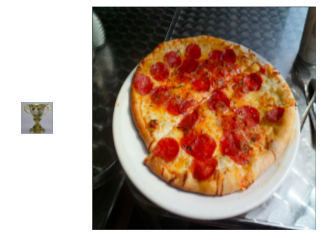
\includegraphics[width=1\textwidth]{recursos/imagens/project/dataset_diff.png}

    Fonte: do próprio autor.
\end{figure}

Além disso, vale citar que a quantidade de informação a ser preservada em pequenos exemplo torna-se mínima, como foi o caso de uso com o conjunto de dados CIFAR 100, contribuindo para o fraco desempenho do método BPCAPooling, mas não sendo uma barreira significativa para os outros métodos de \textit{pooling} tradicionais testados, uma vez que a preservação da espacialidade da amostra de entrada não é a principal preocupação dos métodos \textit{Max Pooling} e \textit{Avg Pooling}.

No processo de \textit{fine-tuning} é possível observar que os conjuntos de treinamento e validação do BPCAPooling mostram uma tendência ascendente, indicando que melhorias adicionais poderiam ser alcançadas com mais épocas no quarto bloco, como demonstra a Figura X.

Figura X

Essa ascensão nos leva a entender que as características espaciais provavelmente sejam captadas no quarto bloco de modo que mais épocas poderiam ser empregadas nessa camada, já que o modelo não apresenta caracteristicas de \textit{overffitting}, todavia a condução de épocas adicionais consumiria muitos recursos devido ao custo computacional associado à complexidade do método.

Fazer parâgrafo de conclusão.

\subsubsection{LIME e Preservação de Espacialidade}
\label{results:class:lime}
- Apresentar processo de preservação espacial, lime, fine tunning e custo computacional.

\subsubsection{Trabalhos Futuros}
\label{results:class:future}
- Será que o uso de transferência de aprendizado foi bom nesse caso? Pois as camadas de pooling não têm parâmetros, mas a atuação das mesmas acabam influenciando as demais camadas.

\subsection{Resultados da Segmentação Semântica}
\label{results:semantic}
- Colocar imagem para cada um dos resultados dos modelos e falar sobre a baixa diferença visualmente falando (falar que a diferença será relatada na seção \ref{results:semantic:xai})
- Não há uma discrepância significativa em relação às métricas quando comparado com max pooling, mas se apresenta mais lento e ainda tem menores métricas.
- Na prática em relação não tem muita mudança no resultado final exceto pelo tempo, complexidade e baixa acurácia

\subsubsection{Diferença das arquiteturas}
\label{results:semantic:arch}
- O treinamento com U-Net-Like realmente ocorrem mais rápido do que as U-Nets convencionais, visto que a quantidade de parâmetros é menor e as normalizações de batch normalization e convolução separáveis trazem o beneficio das otimizações.

\subsubsection{Explicação de modelos}
\label{results:semantic:xai}
- Colocar imagens comparando, mostrar os pontos de maior diferença para BPCA e Max Pooling.

\subsubsection{Trabalhos Futuros}
\label{results:semantic:future}
- Propor o uso de outro framework como pytorch e falar dos problemas tecnicamente enfrentados.
- Valeria um teste com outros datasets contendo objetos de diversos tamanhos, como lost and found, cityscape ou celulas. Mas a adaptação de código com o framework tensforflow se torna custosa, valeria a migração para o pytorch tentando minimizar essa barreira tecnológica.
- Valeria a implementação de um método de unpooling com o processo reverso de bpca (colocar a fórmula e imagens (repo compartilhado com uemerson)), a diferença é que esse método contaria com parâmetros, sendo necessário usar uma camada densa por baixo dos panos.


\subsection{Considerações Finais do Capítulo}
\label{result:final}
